\documentclass[a4paper,12pt]{article}
\usepackage[utf8]{inputenc}
\usepackage[T1]{fontenc}
\usepackage[slovene]{babel}
\usepackage{graphicx}

\title{Računalniški praktikum II}
\author{Naloga za samostojno reševanje 3}
\date{15. marec 2019}

\begin{document}
\maketitle
\thispagestyle{empty}

\noindent
V jeziku HTML izdelajte spletni obrazec za vnos podatkov o študentu, kot je prikazan na spodnji sliki. [0.5~točke]
\begin{center}
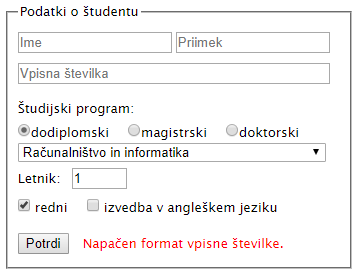
\includegraphics{obrazec.png}
\end{center}

\noindent
V jeziku JavaScript sestavite ustrezne funkcije, ki ob pritisku na gumb `Potrdi' preverijo pravilnost vnosa podatkov glede na sledeče kriterije: [1.5~točke]
\begin{itemize}
\item Ime in priimek sta obvezna podatka.
\item Vpisna številka je obvezen podatek. Sestavljena je iz niza osmih števk, ki se začne z `89'.
\item Dodiplomski in doktorski študij obsegata tri letnike, magistrski dva letnika.
\item Izredni študij se izvaja le v slovenskem jeziku.
\item Obvestilo o napaki naj se izpiše ob gumbu `Potrdi'.
\end{itemize}
\end{document}